\documentclass[review]{elsarticle}
\usepackage[utf8]{inputenc}
\usepackage{amsmath}
\usepackage{amssymb}
\usepackage{tabularx}
\usepackage{multirow}
\usepackage{multicol}
\usepackage{array}
\usepackage{longtable} %continued float
\usepackage{siunitx}
\usepackage{booktabs}
\bibliographystyle{elsarticle-num}
\usepackage{lineno,hyperref}
\modulolinenumbers[5]
\usepackage{graphicx}
\usepackage{algorithm}
\usepackage[noend]{algpseudocode}
\usepackage{caption} % for '\ContinuedFloat' directive
%\usepackage[colorlinks,allcolors=blue]{hyperref}
\usepackage[noabbrev,nameinlink]{cleveref} 
%\usepackage[noabbrev,nameinlink]{cleveref} 
\usepackage[a4paper, total={6in, 8in}]{geometry}
\makeatletter
\def\BState{\State\hskip-\ALG@thistlm}
\makeatother
\usepackage{algpseudocode}

\begin{document}

\title{Write a Paper in LaTeX}
\author[1]{Rohit Salgotra\corref{mycorrespondingauthor}}
\cortext[mycorrespondingauthor]{Corresponding author}
\ead{r.03dec@gmail.com}
\address[1]{Dept. of LaTeX Studies}
\date{June 2024}

\author[2]{Xy Zy}
\ead{notmyemail@gmail.com}
\address[2]{Dept. of Not Studying At All}
%-----------Abstract ------%
\begin{abstract}
 This is how we write a paper in Latex...!!
\end{abstract}
\maketitle

\section{Introduction}


\textbf{Research is a systematic and methodical process of investigating specific questions, issues, or phenomena to acquire new knowledge or validate existing theories \cite{das2010differential}.}


\textbf{\textit{"It encompasses various approaches, including qualitative, quantitative, and mixed-methods, each suited to different types of inquiries \cite{salgotranaked}." }}


\textcolor{red}{Researchers employ a range of techniques such as experiments, surveys, case studies, and archival research, guided by clear hypotheses or research questions \footnote{Automatically generated footnote markers work fine!}. }


Effective research requires:
\begin{itemize}
    \item critical thinking
    \item rigorous methodology
    \item ethical considerations to ensure accuracy
    \item reliability
    \item integrity of the findings
\end{itemize}

In section \ref{section:2}, equations are there; section \ref{section:4} tables are there; and in section \ref{section:3} figures are there.


\section{Define an equation} \label{section:2}

We can make equations from here : \href{https://latex.codecogs.com/eqneditor/editor.php}{https://latex.codecogs.com/eqneditor/editor.php}

\subsection{Basic Maths}
a=b+c

\subsubsection{in Signs}
$a= b+c$

$x_1^3 = x_1 + y^2$


\subsection{Advanced}
using equation \ref{eq:1}



\begin{equation}
    f(x) = \sum_{n=1}^{T+1}   \label{eq:1}
\end{equation}

\begin{equation}
    x_1^3 = x_1 + y^2 \label{eq:2}
\end{equation}


$x_{best}^{t+1} = r^{ier}_{heuwfh} + r{ehwi}^b{jfsefb}$

\begin{equation}
    x_{be,st}^{t+1} = r^{ier}_{heuwfh} + r{ehwi}^b{jfsefb}
\end{equation}
\section{Tables in LaTeX} \label{section:4}

Drawing tables is very difficult as shown in Table \ref{Table:1}. But there is a rescue:

We can go to \href{https://www.tablesgenerator.com/}{https://www.tablesgenerator.com/}


% Please add the following required packages to your document preamble:
% \usepackage{multirow}
\begin{table}[h]
\caption{This is the first table} \label{Table:1}
\centering
\begin{tabular}{lllll} \hline
a                 & b & \multicolumn{2}{l}{c}             & d             \\ \hline
\multirow{2}{*}{1} &  1 &        2   &               3        &     4          \\ \cline{2-5}
                  & 4  &       5    & \multicolumn{2}{l}{\multirow{2}{*}{}} 3\\ \hline
                  &   &     4      & \multicolumn{2}{l}{5}   \\ \hline            
\end{tabular}

\end{table}

\section{Figures in LaTeX} \label{section:3}

Lets add a figure here \ref{fig:1}. 


\begin{figure}[ht]
    \centering
    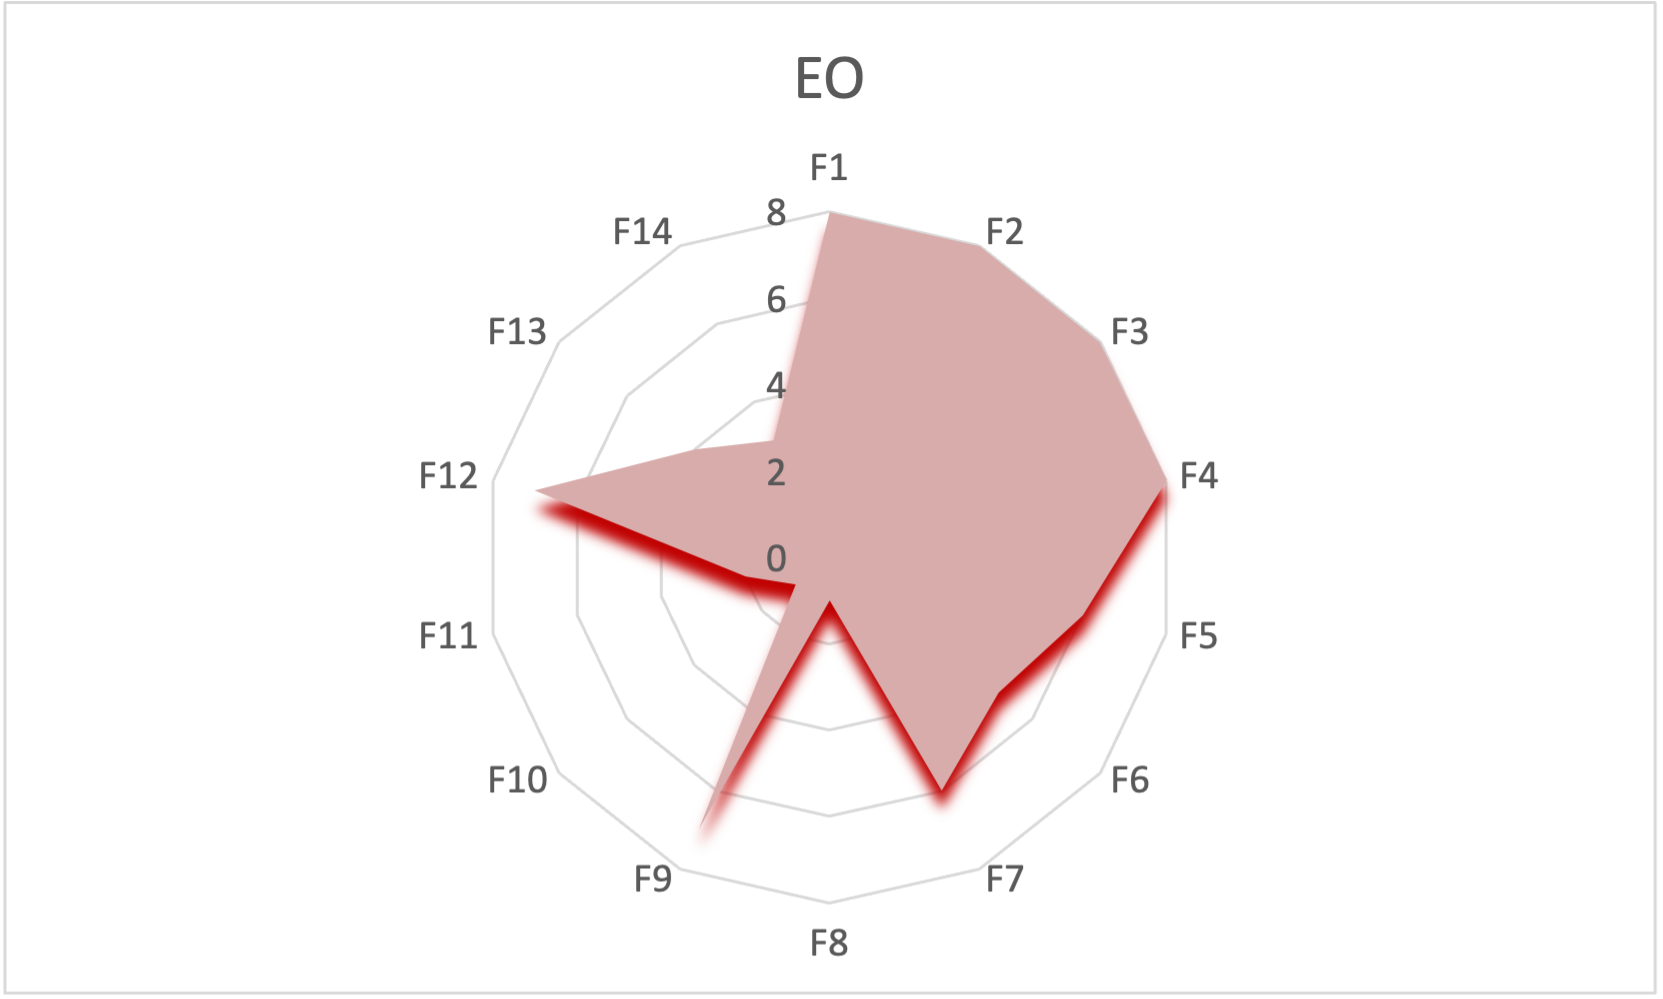
\includegraphics[width=0.8\textwidth]{EO.png}
    \caption{This is my Figure} \label{fig:1}
\end{figure}


\section{Conclusion} \label{section:5}

$\alpha$, $\beta$, $\gamma$ are they symbols, and you can find them at: 

\href{https://oeis.org/wiki/List_of_LaTeX_mathematical_symbols}{Click to get the symbols}




\bibliography{Bibliography}
\end{document}
